% <<FF>> ***********************************************************************
% https://www.overleaf.com/learn/latex/Beamer_Presentations:_A_Tutorial_for_Beginners_(Part_2)%E2%80%94Lists,_Columns,_Pictures,_Descriptions_and_Tables#The_Description_Environment
\begin{frame}
  \frametitle{A motivating Example for SMC}

 \begin{columns}
   \column{0.5\textwidth}
   Sliding mode of the system:

   \begin{equation}
   \ddot x = \sin(3 t) + u 
   \end{equation}
     \column{0.5\textwidth}
   \centering
    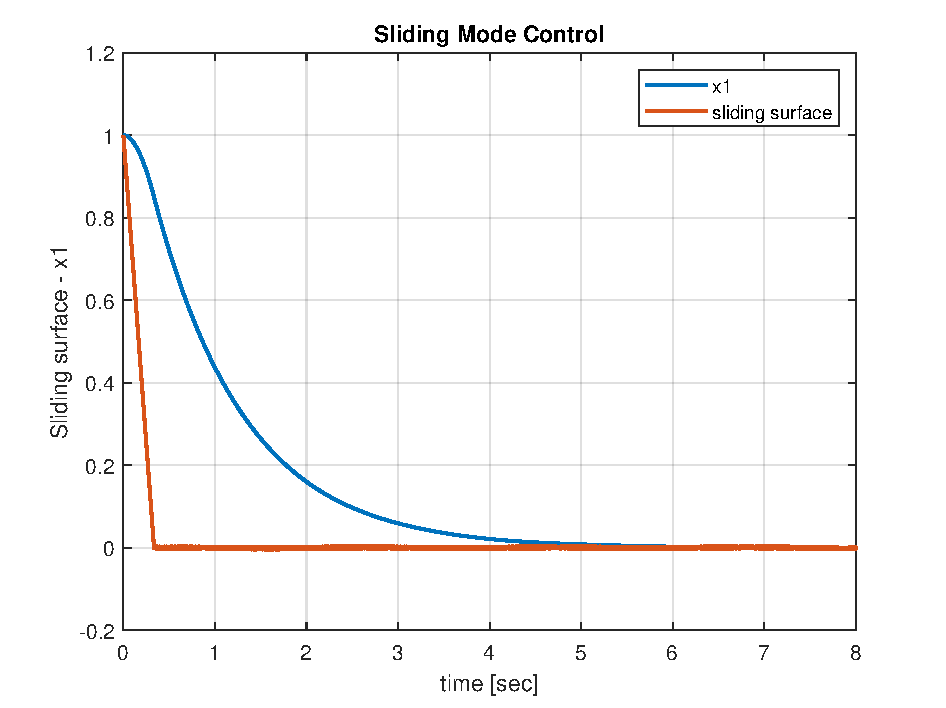
\includegraphics[height=4cm]{./pictures/SMCutkinRoadmap.pdf}
\end{columns}
 \end{frame}
%%% Local Variables:
%%% mode: latex
%%% TeX-master: "SMC4Students"
%%% End:
